\documentclass[english,12pt,a4paper]{report}
% permet l'utiliation des \subsubsection{}
\setcounter{secnumdepth}{4}
% ajout des subsubsection dans la table de matère
\setcounter{tocdepth}{4}
\usepackage[utf8]{inputenc}
\usepackage[T1]{fontenc}
\usepackage{amsmath}
\usepackage{amssymb}
\usepackage{graphicx}
\usepackage[top=1.5cm,bottom=2cm,left=2cm,right=2cm]{geometry}
\usepackage{array}
\usepackage{multirow}
\usepackage{multicol}
\usepackage{enumerate}
\usepackage{layout}
\usepackage{dirtytalk}
\usepackage{setspace}
\usepackage{sectsty}
\usepackage{float}
\usepackage{gensymb}
\usepackage{tikz}
\usepackage{enumitem}
\usepackage{listings}
\usepackage{comment}
\usepackage{caption}
\usepackage{subcaption}
\usepackage{fancyhdr}
\usepackage{blindtext}
\usepackage{parskip}
\usepackage{babel}
\usepackage{hyperref}
\setlength{\parindent}{4em}
\setlength{\parskip}{1em}
\chapterfont{\centering}
\pagestyle{fancy}
\fancyhf{}
\fancyheadoffset{0cm}
\renewcommand{\headrulewidth}{0pt}
\renewcommand{\footrulewidth}{0pt}
\fancyhead[R]{\thepage}
\fancypagestyle{plain}{\fancyhf{}\fancyhead[R]{\thepage}}
\begin{document}
\begin{spacing}{1.5}
\begin{titlepage}
\begin{center}
\begin{center}
\begin{tabular}{c c c}
	REPUBLIQUE DU CAMEROUN &             & REPUBLIC OF CAMEROON\\
	Paix-Travail-Patrie &             & Peace-Work-Fatherland\\
	\vspace{1cm} 
	MINESEC &             & MINESEC\\
	DELEGATION DEPARTEMENTALE  &             & MENOUA DIVISIONAL \\
	DE LA MENOUA &             & DELEGATION \\
	LYCEE CLASSIQUE DE DSCHANG &   \hspace{3cm}          & DEPARTEMENT D'INFORMATIQUE
\end{tabular}
\end{center}
\vspace{1.5cm}
{\huge\scshape\textbf{RAPPORT DE STAGE}}\\
\vspace{1.5cm}
{{\Large\scshape\textbf{THEME: UNE APPLICATION DESKTOP POUR LA GESTION DES EMPLOIES DE TEMPS SCOLAIRE}}\\{\Large Redigé et presenté \emph{par: }\\
\textbf{KAMSU MODJO\emph{(230968817)}\\} \textbf{TATANG NGUENA\emph{(231305012)}}\\}}
\vspace{1.2cm}
{\large{Ce projet soumis au collège de formation des enseignants d'informatiques du lycée classique de Dschang dans le cadre de l'obtention partielle du BACCALAUREAT ESG de la série TI(technologie de l'information)}\\}
\vspace{1cm}
{\large Supervisé \emph{par:}
\textbf{Mr. GOUFACK}\\
\large co-encadré \emph{par:}
\textbf{Mr. ELLA EMMANUEL}}
\vfill
{\itshape Mai, 2025}
\end{center}
\end{titlepage}
\cleardoublepage
\pagenumbering{roman}
\addcontentsline{toc}{chapter}{CERTIFICATION}
\chapter*{CERTIFICATION}
\hspace{1.2cm}
Nous attestons que ce projet intitulé << UNE APPLICATION DESKTOP POUR LA GESTION DES EMPLOIE DE TEMPS SCOLAIRE>> a été réalisé par \textbf{KAMSU MODJO YVAN} et \textbf{TATANG NGUENA} avec les numéro de matricule 230968817 et 231305012 de la série Technologie de l'information du département d'informatique du lycée classique de Dschang.
\begin{center}
	\vspace{0.2cm}
	\emph{Encadreur}\\
	\vspace{0.2cm}
	\textbf{Mr. GOUFACK}\\
	\vspace{0.2cm}
	Date:
	\begin{tikzpicture}
		\draw(0,0)--(4,0);
	\end{tikzpicture}\\
	\vspace{0.2cm}
	\emph{Co-Encadreur}\\
	\vspace{0.2cm}
	\textbf{Mr. ELLA EMMANUEL}\\
	\vspace{0.2cm}
	Date:
	\begin{tikzpicture}
		\draw(0,0)--(4,0);
	\end{tikzpicture}\\
	\vspace{0.5cm}
	\emph{Animateur Pédagogique}\\
	\vspace{0.2cm}
	\textbf{Mr. ELLA EMMANUEL}\\
	\vspace{0.2cm}
	Date:
	\begin{tikzpicture}
		\draw(0,0)--(4,0);
	\end{tikzpicture}
\end{center}
\addcontentsline{toc}{chapter}{ATTESTATION}
\chapter*{ATTESTATION}
\hspace{1.2cm}
C'est avec beaucoup d'enthousiasme que nous sommes les auteurs de ce projet << UNE APPLICATION DESKTOP POUR LA GESTION DES EMPLOIES DE TEMPS SCOLAIRE >> et nous donnons la permission au lycée classique de Dschang, par l'intermédiaire du département d'informatique, de prêter ce projet à d'autres établissements scolaires ou individus à des fins de recherche académique. Nous comprenons la nature du plagiat et nous somme conscients de la politique éducative à ce sujet; nous somme convaincus que ce sujet est original et réalisé par nous au cours de nos étude pour l'obtention du BACCALAUREAT ESG en Technologie de l'information.
\begin{center}
\vspace{1cm}
\vspace{0.2cm}
\textbf{KAMSU MODJO YVAN}\\
\textbf{TATANG NGUENA}\\
\vspace{0.2cm}
Date:
\begin{tikzpicture}
	\draw(0,0)--(4,0);
\end{tikzpicture}\\
\vspace{0.2cm}
Signature:
\begin{tikzpicture}
	\draw(0,0)--(4,0);
\end{tikzpicture}
\end{center}
\phantomsection
\addcontentsline{toc}{chapter}{DEDICACE}
\chapter*{DEDICACE}
\hspace{1.2cm} 
\begin{center}
	\textbf{nous dédions ce travail à nos parents}
\end{center}
\vspace{-1.5cm}
\addcontentsline{toc}{chapter}{REMERCIEMENT}
\chapter*{REMERCIEMENT}
\vspace{-1.5cm}
\hspace{1.cm}
le mérite d'un travail ne revient pas toujours systématiquement à ses seuls acteurs. Nous ne pouvions donc pas conclure un tel ouvrage sans saluer les efforts de certaines personnes qui nous ont aidés et guidés de diverses manières. c'est pourquoi nous tenons à leur exprimer notre profonde gratitude, en particulier:
\begin{itemize}[label=\textbullet, font=\LARGE %\color{blue}
	]
	\item Le proviseur du Lycée Classique de Dschang - \textbf{Mr ATEM NDE JEAN CLAUDE} qui a permis toutes les nécessités pour notre meilleure formation.
	
	\item Le Censeur en charge de l'informatique - \textbf{Mr TEMGOUA} pour sa faculté à nous trouver du stage et à veiller qu'on reçoivent de bon enseignements.
	
	\item L'animateur Pédagogique \textbf{Mr ELLA EMMANUEL}, Un modèle à suivre, pour nous avoir aider et guider tout au long de notre formation.
	
	\item Notre encadreur  \textbf{	Mr GOUFACK }  pour ses conseils   
	
	\item Notre co-encadreur \textbf{Mr. ELLA EMMANUEL } Pour sa supervision, sa disponibilité et ses conseils lors de notre formation  et pour sa supervision 
	
	
	\item du personnel administratif, le Collège des enseignants du lycée classique de Dschang en général et les enseignants du département d'informatique en particulier;
	
	\item Tous les membres du jury qui ont pris leur temps précieux pour lire et nous aider à améliorer ce travail ; 
	
	\item 	 Nos parents, pour leur esprit de sacrifice, leur soutien financier et moral ainsi que leurs conseils et encouragements
	\item 	 à tous nos camarades de classe qui ont créé autour de nous une excellente ambiance de travail
	\item 	 nous remercions également ceux dont les noms ne sont pas mentionnés ici, pour leur aide
\end{itemize}	

\addcontentsline{toc}{chapter}{RESUME}
\chapter*{RESUME}
\hspace{1.2cm}
Dans un établissement scolaire, la gestion des emplois du temps est une tâche complexe qui nécessite une organisation rigoureuse. Un mauvais agencement des horaires peut entraîner des conflits entre les enseignants, les salles de classe et les matières enseignées.

L’objectif de ce projet est de développer une application de gestion des emplois du temps, permettant d’optimiser la planification des cours en fonction des disponibilités des professeurs, des salles et des classes. Cette application, développée en JavaFX et l'IDE Eclipse avec une base de données SQLite, vise à automatiser la création et la gestion des emplois du temps pour améliorer l’efficacité et réduire les erreurs humaines.

Ce rapport présente l’analyse du projet, les acteurs impliqués, ainsi que l’étude de faisabilité technique et organisationnelle.
\bigskip 
\bigskip
\par 

%\textbf{Mots-clés:} IMMOBIZ, application mobile, Android, immobilier
\addcontentsline{toc}{chapter}{ABSTRACT}
\chapter*{ABSTRACT}
\hspace{1.2cm}
In a school setting, timetable management is a complex task requiring rigorous organization. Poor scheduling can lead to conflicts between teachers, classrooms, and subjects taught.

The goal of this project is to develop a timetable management application to optimize class scheduling based on teacher availability, classroom availability, and class groups. This application, developed in JavaFX with an SQLite database, aims to automate timetable creation and management to improve efficiency and reduce human errors.

This report presents the project analysis, involved stakeholders, and the technical and organizational feasibility study.


\bigskip 
\bigskip
\par 

\textbf{Keywords:} IDE, JavaFX, application desktop, 
\addcontentsline{toc}{chapter}{LISTE DES ABRÉVIATIONS}
\chapter*{LISTE DES ABRÉVIATIONS}
\textbf{IDE} : Integrated Development environment 

\textbf{OS} : 	 Operating System 

\textbf{SQL} :  	Structured Query Language

\textbf{UML} : Unified Modeling Language

\textbf{CSS} : Cascading StyleSheets
\end{spacing}

\tableofcontents

\cleardoublepage
\phantomsection

\addcontentsline{toc}{chapter}{LISTE DES FIGURES}
\listoffigures

\cleardoublepage
\phantomsection

\addcontentsline{toc}{chapter}{LISTE DES TABLEAUX}
\listoftables


\addcontentsline{toc}{chapter}{INTRODUCTION GENERALE}


\chapter*{INTRODUCTION GENERALE}
\vspace{0.8cm}
\pagenumbering{arabic}

\section{contexte}
Dans un monde en constante évolution, l'organisation et la gestion efficace du temps sont devenues des enjeux majeurs pour les établissements scolaires. L'emploi du temps constitue un élément fondamental du bon fonctionnement d'un établissement, permettant de structurer les activités pédagogiques, d'optimiser l'utilisation des ressources et d'assurer un équilibre entre les contraintes des enseignants, des élèves et des infrastructures disponibles. Cependant, la planification et la gestion manuelle des emplois du temps peuvent s'avérer complexes et chrono-phages, entraînant des conflits d'horaire, une mauvaise allocation des salles et une difficulté à répondre aux imprévus. Pour pallier ces problématiques, l'intégration d'un système informatisé devient une nécessité afin d'automatiser et de simplifier ces processus.

C’est dans cette optique que notre projet de gestion des emplois du temps a été conçu. Il vise à fournir une solution logicielle efficace permettant aux administrateurs scolaires de créer, modifier et consulter les emplois du temps en toute simplicité. Ce système offrira également aux enseignants et aux responsables pédagogiques un accès rapide aux informations essentielles, facilitant ainsi la coordination et l’organisation des cours. À travers ce rapport, nous présenterons l’ensemble des aspects liés à la conception, au développement et à la mise en œuvre de cette application, en mettant l’accent sur les besoins des utilisateurs, les choix technologiques et les bénéfices attendus.

\section{La problématique}
Dans un établissement scolaire, la gestion des emplois du temps est un processus essentiel mais souvent complexe. Entre la disponibilité des enseignants, la répartition des salles, la prise en compte des différentes disciplines et les contraintes spécifiques de chaque niveau d’enseignement, l’élaboration d’un emploi du temps optimal devient un véritable casse-tête. Les méthodes traditionnelles, souvent basées sur des tableaux manuels ou des fichiers Excel, sont limitées et sujettes aux erreurs : chevauchements d’horaires, mauvaise allocation des ressources, difficultés d’adaptation aux imprévus (absences, changements de salle, etc.). De plus, l’absence d’un système centralisé complique l’accès et la mise à jour rapide des informations pour les différents acteurs de l’établissement. Ainsi, la question centrale que soulève ce projet est la suivante :
\textbf{Comment concevoir et mettre en place un système informatisé permettant une gestion efficace, flexible et automatisée des emplois du temps dans un établissement scolaire, tout en assurant un accès rapide et structuré aux informations pour les administrateurs, enseignants et autres parties prenantes ?} Ce projet vise donc à proposer une solution logicielle innovante permettant d’optimiser la planification des emplois du temps tout en réduisant les erreurs humaines et en améliorant la coordination entre les acteurs concernés

\section{Objectifs du projet }
 L’objectif principal de ce projet est de concevoir et développer une application informatique de gestion des emplois du temps pour un établissement scolaire, permettant une planification efficace et automatisée des cours, des enseignants et des salles
 Pour atteindre l'objectif standard, les objectifs suivants doivent être poursuivis : 
\begin{itemize}
	\item Automatiser la planification des emplois du temps afin de réduire les erreurs humaines et optimiser l’organisation des cours.
	\item Faciliter l’accès aux informations pour les différents acteurs (administrateurs, enseignants, responsables des emplois du temps) grâce à une interface intuitive et centralisée
	\item Gérer dynamiquement les imprévus tels que les absences des enseignants ou l’indisponibilité des salles, en permettant des mises à jour rapides et efficaces.
	\item Garantir une meilleure organisation des ressources (enseignants, salles, disciplines) afin d’éviter les conflits d’horaires et d’améliorer l’efficacité du système éducatif.
	\item Proposer un accès sécurisé et différencié selon le rôle de l’utilisateur (administrateur, responsable des emplois du temps, professeur).
\end{itemize}

\subsection{Objectif général du projet}

L'objectif général de cette étude est de concevoir et de créer une application de bureau pour faciliter la gestion des emploie de temps dans un établissement scolaire.

\subsection{Objectifs spécifiques}
Notre système doit être en mesure de faire ce qui suit:
\begin{itemize}
	\item Gérer les ressources : Professeurs, classes, matières et salles de cours.
	\item Éviter les conflits d’horaires en assurant une bonne répartition des cours et des salles.
	\item Offrir une interface intuitive pour que les administrateurs, enseignants et élèves puissent consulter les emplois du temps.
	\item Faciliter les modifications et mises à jour en cas de changements de dernière minute.
	\item déterminer s'il existe une disparité dans les valeurs locatives des propriétés résidentielles et commerciales dans la zone d'étude.
	
\end{itemize}


\section{Importance du projet }
La mise en place d’une application de gestion des emplois du temps revêt une importance capitale pour un établissement scolaire. En effet, la gestion manuelle des emplois du temps est souvent source d’erreurs, de conflits d’horaires et de pertes de temps considérables. Ce projet apporte donc plusieurs avantages :

\begin{itemize}
	\item \textbf{Optimisation de la gestion des emplois du temps} : L’automatisation permet d’attribuer efficacement les cours aux enseignants et aux salles tout en respectant les contraintes pédagogiques et administratives.
	\item \textbf{Réduction des erreurs humaines} : En évitant les conflits d’horaires, les doubles affectations et les oublis, l’application garantit une meilleure organisation.
	\item \textbf{Gain de temps} : La génération automatique des emplois du temps réduit le travail manuel fastidieux, permettant ainsi aux administrateurs et responsables de se concentrer sur d’autres tâches essentielles.
\end{itemize}

\section{Le plan de rédaction }

Ce travail est structuré comme suit :

\begin{itemize}
	\item 	\textbf{Introduction générale} Cette section présente le contexte général du projet, la problématique liée à la gestion manuelle des emplois du temps, les objectifs poursuivis, l’importance du projet pour l’établissement, ainsi qu’un aperçu global du contenu du rapport.
	
	\item 	 \textbf{Le premier chapitre intitulé « étude de l'existant »} Cette partie analyse l’organisation actuelle de la gestion des emplois du temps dans l’établissement, expose les difficultés rencontrées avec le système manuel, propose des définitions clés, et inclut une revue de la littérature sur les solutions similaires existantes dans d’autres contextes éducatifs.
	
	\item  \textbf{chapitre2: Analyse et Conception} Ce chapitre décrit les méthodes d’analyse (Merise, UML) utilisées pour comprendre les besoins fonctionnels et techniques du système, et présente les différents diagrammes de conception : cas d’utilisation, diagrammes de classes, MCD, MLD, etc. Il constitue la base de réflexion pour la modélisation de l'application.
	
	\item 	\textbf{chapitre 3: Implémentation}: On y détaille les outils matériels et logiciels utilisés (langage de programmation, base de données, IDE, bibliothèques), l’architecture de l’application, les principales fonctionnalités implémentées, ainsi que les interfaces graphiques développées.;
	
	\item  \textbf{La dernière section intitulée « Conclusion et recommandations »} constituait le résumé des conclusions et recommandations. 
\end{itemize}

% --------------premier chapitre
\addcontentsline{toc}{chapter}{ÉTUDE DE L'EXISTANT}
\chapter{ÉTUDE DE L'EXISTANT}
\section{Présentation de l'établissement}
L’établissement scolaire concerné est le lycée classique de Dschang accueillant plusieurs centaines d’élèves répartis dans différentes classes, filières et niveaux. Le corps enseignant est composé d’enseignants permanents et vacataires, encadrés par une équipe administrative comprenant notamment le proviseur, les censeurs, et les surveillants généraux.
L’organisation pédagogique repose sur une répartition hebdomadaire des cours selon les disponibilités des professeurs, les ressources matérielles (salles de classe, laboratoires) et les contraintes pédagogiques propres à chaque filière.

\section{Organisation actuelle de la gestion des emplois du temps}
Actuellement, la gestion des emplois du temps est assurée manuellement par le personnel administratif, notamment le censeur chargé de la pédagogie. Celui-ci utilise principalement des outils bureautiques comme Microsoft Excel ou parfois même des feuilles papier pour planifier les horaires.
Chaque emploi du temps est élaboré à la main en prenant en compte les disponibilités des enseignants, la répartition horaire des matières par semaine, les salles disponibles, et les contraintes de chevauchement. Une fois les plannings validés, ils sont imprimés et affichés dans les salles de classe.

\section{Outils utilisés}
\begin{itemize}
	\item \textbf{Feuilles de calcul Excel} pour structurer les emplois du temps.
	\item \textbf{Documents papier} pour les premiers brouillons et modifications manuelles.
	\item \textbf{Communication orale} ou via messagerie interne pour informer les enseignants en cas de changement.
	\item \textbf{Aucune base de données centralisée} n'est utilisée actuellement pour stocker les informations des enseignants, des classes ou des salles.
\end{itemize}

\section{Difficultés et limites du système actuel}
La gestion manuelle présente de nombreuses limites:
\begin{itemize}
	\item Erreurs humaines fréquentes (conflits d’horaires, doublons, oublis).
	\item Temps de traitement très long à chaque rentrée ou changement de planning.
	\item Difficulté à modifier ou ajuster rapidement les emplois du temps.
	\item Aucune automatisation des vérifications (disponibilité des profs, nombre d’heures, chevauchements).
	\item Manque de traçabilité et d’archivage des emplois du temps précédents.
\end{itemize}

\section{Besoin d’un système informatisé}
Pour répondre aux limites évoquées, il est essentiel de mettre en place un système informatisé permettant de :
\begin{itemize}
	\item Automatiser la création des emplois du temps.
	\item Réduire les erreurs grâce à des vérifications automatiques.
	\item Rendre l’accès aux emplois du temps plus simple et rapide, y compris pour les élèves et les enseignants.
	\item Générer des exports PDF ou des impressions propres et formatées.
\end{itemize}
Le développement d’une application dédiée répond donc à un besoin réel \textbf{d’optimisation et de modernisation} de la gestion scolaire, tout en améliorant le quotidien des personnels administratifs.

% ----------------- chapitre 2
\addcontentsline{toc}{chapter}{ANALYSE ET CONCEPTION}
\chapter{ANALYSE ET CONCEPTION}
\section{ANALYSE}
Cette partie a pour objectif la spécification de manière claire de l’application. Pour ce faire, il est nécessaire de déterminer globalement ce qui se trouve dans le champ de l’application. De ce fait, on s’intéressera dans cette phase à l’identification des acteurs du système, leurs espaces et le contexte de l’application.
\subsection{IDENTIFICATION DES ACTEURS DE L'APPLICATION}
Pendant l’étude qu’on a effectuée, nous avons procédé à l’identification des
principaux acteurs qui seront les futurs utilisateurs de l’application, ces acteurs
sont :
\begin{itemize}
	%---------- admin
	\item \textbf{l'administrateur}
	\begin{itemize}
		\item Gestion des utilisateurs
		\item Gestion des Enseignants
		\item Gestion des classes
		\item Gestion des cours
	\end{itemize}
	%--------- responsable du temps
	\item \textbf{Responsable des emploies de temps}
	\begin{itemize}
		\item Gestion des enseignements
		\item Gestion des disponibilités
		\item  Générer un emploie de temps
		\item Gestion des emploies de temps
	\end{itemize}
	%----------- enseignant
	\item \textbf{Enseignant}
	\begin{itemize}
		\item consulter son emploie de temps
		\item consulter sa disponibilité
	\end{itemize}
\end{itemize}

\subsection{DIAGRAMME DE CONTEXTE}
Le diagramme de contexte est un modèle conceptuel de flux qui permet d’avoir
une vision globale des interactions entre le système et les liens avec
l’environnement extérieur. Il permet aussi de bien délimiter le champ de l’étude. Pour notre cas le contexte est donné par la figure suivante :
% inclusion du diagramme de contexte(img)
\begin{figure}[h]
	\centering
	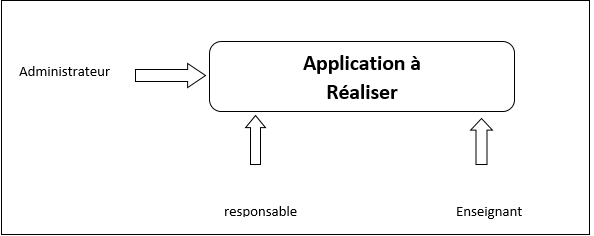
\includegraphics[width=1\textwidth]{dContext.png}
	\caption{Diagramme de contexte}
	\label{fig1: diagramme de contexte}
\end{figure}

\subsection{IDENTIFICATION DES ESPACES}
A chaque acteur est attribué un espace qui regroupe toutes les tâches qu’il peut
effectuer. Pour notre cas nous avons identifié quatre espaces :
\begin{itemize}
	\item Administrateur
	\item Responsable des emploies de Temps
	\item Enseignant
\end{itemize}

\section{CONCEPTION}
C’est la phase la plus complexe du projet. Elle vise principalement à préciser le modèle de telle sorte qu’il puisse être implémenté avec les composantes de l’architecture, pour ce faire nous avons adopté une démarche pour une bonne conception.
\subsection{LA DÉMARCHE DE CONCEPTION DE L'APPLICATION}
Le processus de conception de notre projet se caractérise par deux niveaux : le niveau applicatif et le niveau donné.
\begin{itemize}
	\item \textbf{Niveau applicatif} \par
	S’appuie essentiellement sur quelques diagrammes du langage de modélisation UML. Donc, après avoir identifié les principaux acteurs ainsi que leurs besoins, à travers notre étude, chose qui nous a permis d’identifier les différentes fonctionnalités du système à concevoir, nous avons opté pour la démarche suivante :
	\begin{itemize}
		\item Mettre en évidence les cas d’utilisation mis en œuvre par les utilisateurs futurs du système. Les diagrammes de cas d’utilisation détaillés sont élaborés
		\item A l’aide du diagramme de séquence et d’activité, on formalise graphiquement les scénarios qui décrivent chaque cas d’utilisation.
		\item Les classes sont définies par synthèse des diagrammes de séquence et d’activité. Une fois les classes manipulées sont identifiées, on passe à l’élaboration du diagramme de classe.
	\end{itemize}
	\item \textbf{Niveau donné} \par
	Ce niveau concerne l’organisation conceptuelle, logique et physique des données manipulées. Durant la partie analyse nous avons pu identifier les données nécessaires et indispensables au bon fonctionnement de l’application et à travers la conception du niveau applicatif nous allons dégager les classes significatives. Dès lors on pourra élaborer la conception de la base de données.  La démarche que nous avons adoptée pour la conception de l’application s’appuie sur cinq éléments : \par
	\textbf{1. identification des acteurs et des besoins} \\
	\textbf{2. identification et représentation des cas d’utilisation}\\
	\textbf{3. élaboration des diagrammes de séquences} \\
	\textbf{4. élaboration des diagrammes d’activités}\\
	\textbf{5. élaboration du diagramme de classe} \par
	La figure ci-dessous donne la représentation graphique de la démarche de
	modélisation choisie pour concevoir notre application :
	% inclusion de la demarche de modelisation(img)
	\begin{figure}[h]
		\centering
		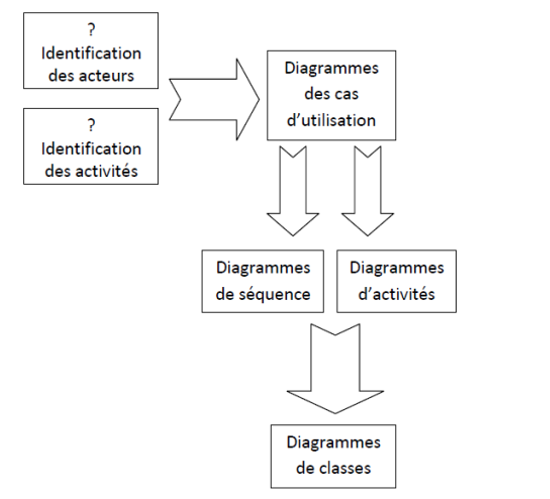
\includegraphics[width=0.6\textwidth]{dContext2.png}
		\caption{Cycle de modélisation de l’application.}
		\label{fig2: Cycle de modélisation de l’application.}
	\end{figure}
\end{itemize}
\subsection{LE NIVEAU APPLICATIF}
\subsubsection{LES CAS D'UTILISATION}
Un cas d’utilisation représente un ensemble de séquences d’actions qui sont réalisées par le système et qui produit un résultat observable intéressant pour un acteur particulier. Il permet de décrire ce que le système devra faire, sans spécifier comment le faire. Dans notre cas nous distinguons les cas d’utilisation suivant :
% listing des different acteur et leur cas d'utilisation
\begin{itemize}
	\item \textbf{Administrateur}
	\begin{itemize}
		\item \textbf{Authentification}
		\item \textbf{gestion des utilisateurs}
		\begin{itemize}
			\item création d'un nouvel utilisateur
			\item modification des informations d'un utilisateur
			\item suppression d'utilisateur
			\item consultation des utilisateurs
		\end{itemize}
		\item \textbf{gestion des enseignants}
		\begin{itemize}
			\item crée un enseignant
			\item modifier les informations d'un enseignant
			\item supprimer un enseignant
			\item consulter un enseignant et son emploie de temps
		\end{itemize}
		\item \textbf{gestion des classes}
		\begin{itemize}
			\item crée une classe
			\item supprimer une classe
			\item modifier une classe
			\item consulter une classe et son emploie de temps
		\end{itemize}
		\item \textbf{gestion des matière}
		\begin{itemize}
			\item crée une nouvelle matière
			\item supprimer une matière
			\item modifier une matière
			\item consulter les matières
		\end{itemize}
	\end{itemize}	
	\item \textbf{Responsable des Emploies du Temps}
	\begin{itemize}
		\item \textbf{Authentification}
		\item \textbf{gestion des enseignements}
		\begin{itemize}
			\item Affecter une matière a un enseignant
			\item modifier
			\item consulter
		\end{itemize}
		\item \textbf{gestion des emploie de temps}
		\begin{itemize}
			\item Générer un emploie de temps
			\item consulter les emploies de temps
		\end{itemize}
		\item \textbf{gestion des disponibilités}
		\begin{itemize}
			\item établir les jours de services d'un enseignant
			\item modifier la disponibilité d'un enseignant
			\item consulter ses jours de services
		\end{itemize}
	\end{itemize}
	\item \textbf{Enseignant}
	\begin{itemize}
		\item \textbf{consulter son emploie de temps}
		\item \textbf{consulter sa disponibilité}
		\item \textbf{consulter ses jours de services}
	\end{itemize}
\end{itemize}
\subsubsection{DIAGRAMME DES CAS D'UTILISATION}
% description et definition du diagramme de cas d'utilisation ici 
Le diagramme de cas d'utilisation est un outil de modélisation appartenant au langage UML (Unified Modeling Language), qui permet de représenter de manière visuelle et synthétique les interactions entre un système et ses utilisateurs, appelés acteurs. Il met en évidence les différentes fonctionnalités que le système propose sous forme de cas d'utilisation, et les relie aux acteurs concernés. 
\begin{figure}[h]
	\centering
	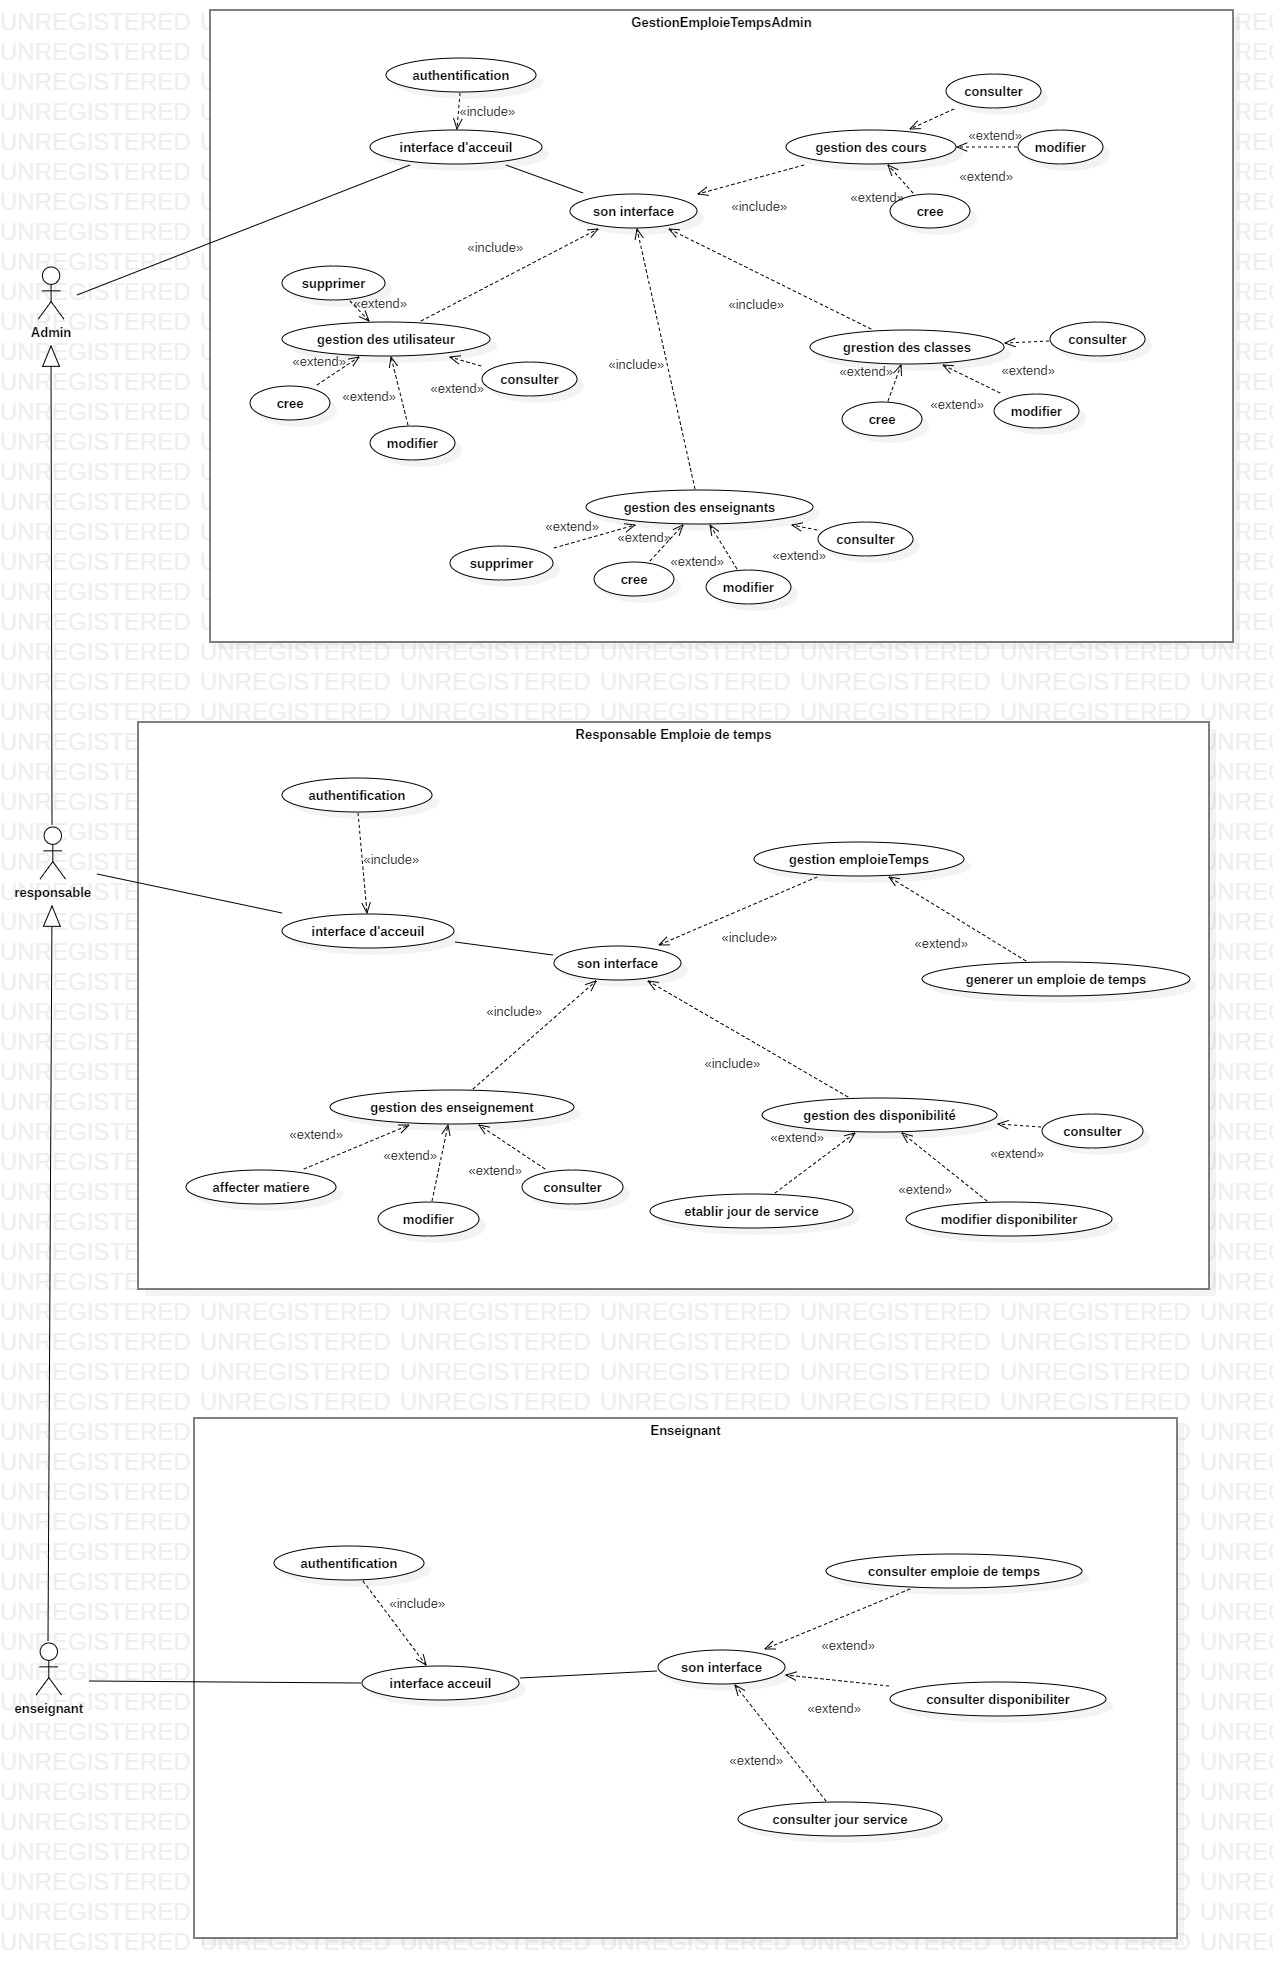
\includegraphics[width=18cm, height=15cm]{UseCaseDiagram1.jpg}
	\caption{diagramme de cas d'utilisation}
	\label{fig3: diagramme de cas d'utilisation}
\end{figure} \par \par
\subsubsection{DIAGRAMME DE SÉQUENCE}
% ddescription du diagramme de sequence ici
Le diagramme de séquence est un type de diagramme UML (Unified Modeling Language) qui permet de représenter de manière chronologique les interactions entre différents éléments d’un système, tels que les objets, les classes ou les acteurs. Il met en évidence l’enchaînement des messages échangés entre ces éléments dans le cadre d’un scénario particulier, tout en respectant l’ordre temporel des actions. Chaque participant est représenté par une ligne de vie verticale, et les échanges sont illustrés par des flèches horizontales. 
\begin{figure}[h]
	\centering
	\begin{center}
		\includegraphics*[height=0.3 \textheight]{AuthentificationSequence.jpg}
	\end{center}
	\caption{diagramme de séquence (Authentification)}
	\label{fig4: diagramme de sequence Authentification}
\end{figure}
\begin{figure}[h]
	\centering
	\includegraphics*[height=0.3 \textheight]{supprimerUtilisateurSequence.jpg}
	\caption{diagramme de séquence (suppression utilisateur)}
	\label{fig5:diagramme de séquence (suppression utilisateur)}
\end{figure}
\begin{figure}[h]
	\centering
	\includegraphics*[height=0.3 \textheight]{creeEmploieTempSequence.jpg}
	\caption{diagramme de séquence (création emploie du temps)}
	\label{fig6:diagramme de séquence (cree emploie du temps)}
\end{figure}
\begin{figure}[h]
	\centering
	\includegraphics*[height=15cm, width=15cm]{consulterEmploiTempSequence.jpg}
	\caption{diagramme de séquence (consulter emploie de temps)}
	\label{fig7:diagramme de séquence (consulter emploie de temps)}
\end{figure}

\clearpage
\subsubsection{DIAGRAMME D'ACTIVITÉ}
Le diagramme d'activité est un type de diagramme UML (Unified Modeling Language) qui permet de représenter de manière détaillée les flux de travail et les processus métier d'un système. Il met en évidence les différentes activités qui sont réalisées, les transitions entre ces activités et les décisions qui sont prises. Chaque activité est représentée par un nœud, et les transitions entre les activités sont illustrées par des flèches. Le diagramme d'activité permet de modéliser les processus métier complexes et de comprendre comment les différentes activités sont liées entre elles. Il est utilisé pour décrire les flux de travail, les processus de prise de décision et les interactions entre les différents éléments du système.
\begin{figure}[h]
	\centering
	\includegraphics*[height=0.5 \textheight]{ActiviteAuthentification.jpg}
	\caption{diagramme d'activité (Authentification)}
	\label{fig8: diagramme d'activité (Authentification)}
\end{figure}
\begin{figure}[h]
	\centering
	\includegraphics*[height=0.7 \textheight]{ActivityCreeEmploieTemps.jpg}
	\caption{diagramme d'activité (création emploie de temps)}
	\label{fig9: diagramme d'activité (creation emploie de temps)}
\end{figure}
\clearpage
\subsubsection{DIAGRAMME DE CLASSE}
Le diagramme de classe est un type de diagramme UML (Unified Modeling Language) qui permet de représenter de manière statique les structures et les relations entre les classes d'un système. Il met en évidence les différentes classes qui composent le système, leurs attributs et leurs méthodes, ainsi que les relations entre ces classes. Chaque classe est représentée par un rectangle, et les relations entre les classes sont illustrées par des lignes et des symboles spécifiques. Le diagramme de classe permet de modéliser les structures de données et les comportements des classes, et de comprendre comment les différentes classes interagissent entre elles. Il est utilisé pour décrire l'architecture logicielle et les relations entre les différents éléments du système.
\begin{figure}[h]
	\centering
	\includegraphics*[height=15cm, width=18cm]{newdiagrammeclasse.jpg}
	\caption{diagramme de classe}
	\label{fig10: diagramme de classe}
\end{figure}



\end{document}